\section{Rigid Material}  This model was designed for use with the
\Textsfc{specified contact} model described in Section~\ref{Sec:Contact}.
It is designed to compute zero stress and identity deformation of the material,
and is basically a fast place-holder for materials that should not develop
any stress.

\begin{lstlisting}[language=XML]
  <constitutive_model type="rigid">
  </constitutive_model>
\end{lstlisting}

\begin{minipage}[t]{0.9\textwidth}
  \centering
  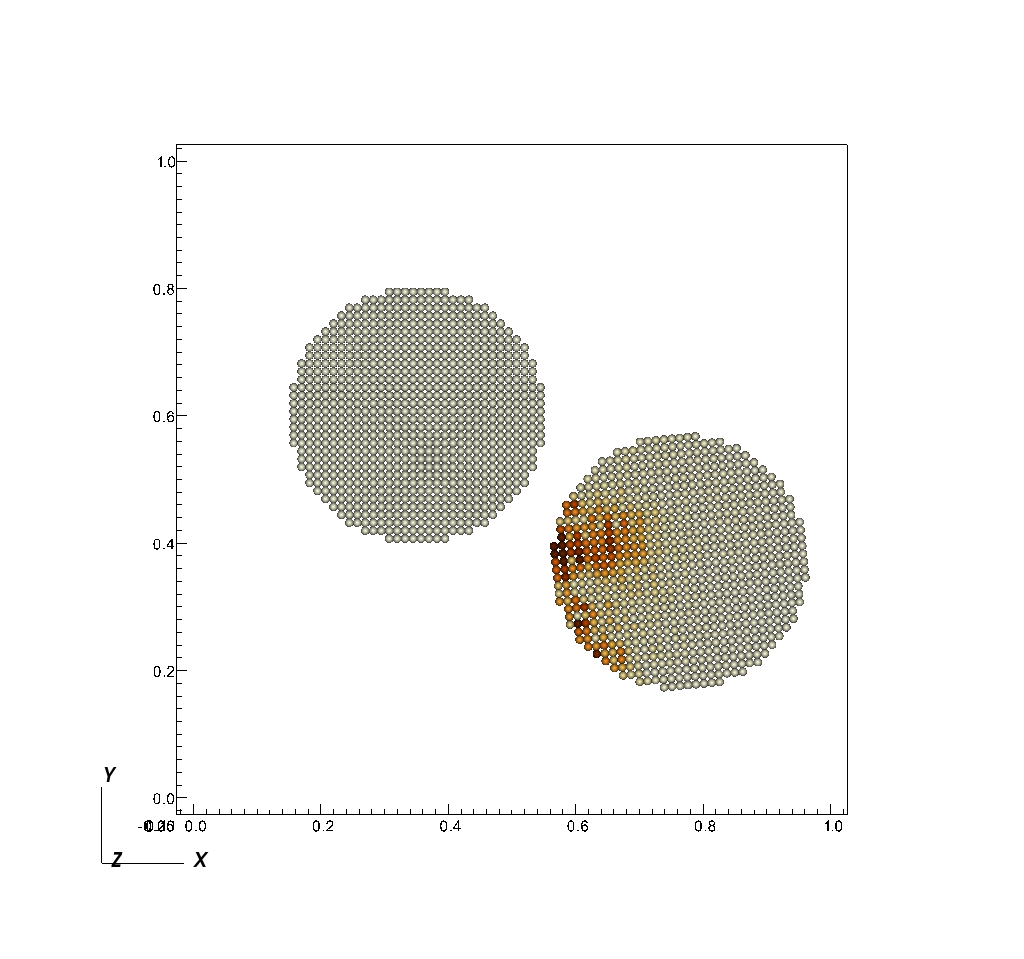
\includegraphics[width=0.5\columnwidth]{FIGS/contact/specified2.png}
  \captionof{figure}{A \Textsfc{rigid} disk (left) interacting with a deformable disk (right).}
\end{minipage}

